%
% orion2.tex
%
% (c) 2023 Prof Dr Adnreas Müller
%
\begin{figure}
\centering
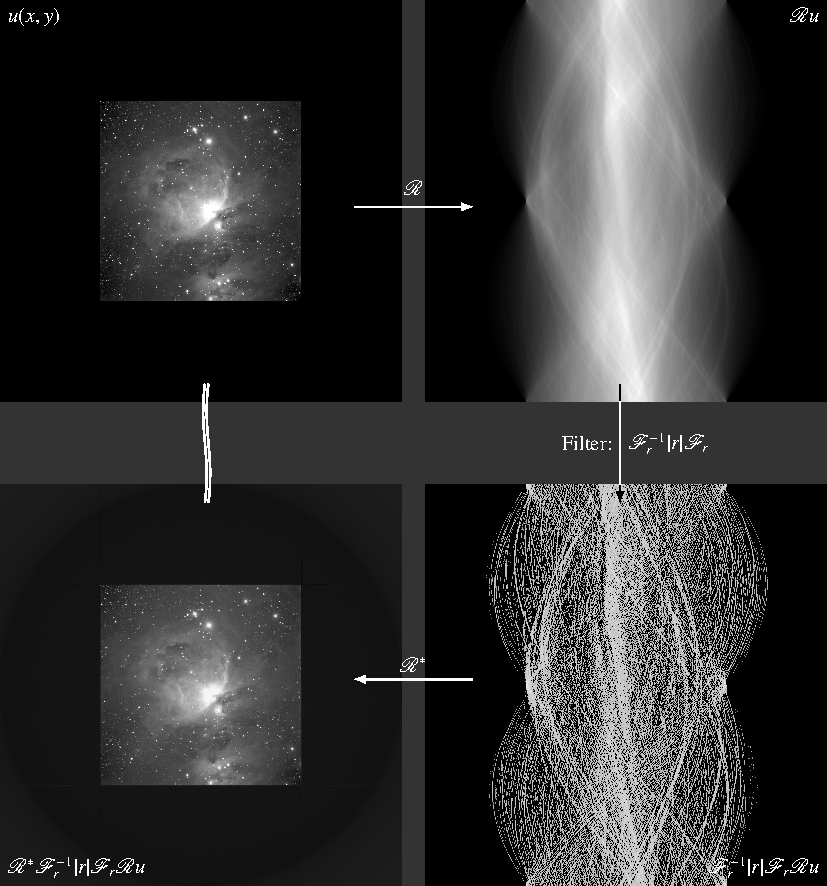
\includegraphics[width=\textwidth]{chapters/050-radon/images/orion2.pdf}
\caption{Rekonstruktion eines Bildes $u$ aus der Radon-Transformierten
$\mathscr{R}u$.
Die Rückprojektion $\mathscr{R}^*\mathbb{R}u$ ist stark verschwommen.
Durch die Anwendung des Filters vor der Rückprojektion kann ein
scharfes und kontrastreiches Bild gewonnen werden.
Die Filterung funktioniert besser, wenn das Bild von einem genügend 
grossen scharzen Gebiet umgeben ist.
\label{buch:radon:rueckprojektion:fig:rueckprojektion}}
\end{figure}
